\documentclass[a4paper,10pt]{article}
\usepackage[utf8]{inputenc}
\usepackage{amsmath}
\usepackage{amssymb}
\usepackage{bm}
\usepackage{caption}
\usepackage{subcaption}
\usepackage{graphicx}

% Operators
\newcommand{\tr}{\mathrm{tr} \hspace{0.05cm} }

% Vectors
% \newcommand{\Xvec}{\bm{X}}
% \newcommand{\xvec}{\bm{x}}
% \newcommand{\uvec}{\bm{u}}
% \newcommand{\ef}{\bm{f}_0}
% \newcommand{\es}{\bm{s}_0}
% \newcommand{\en}{\bm{e}_n}
% \newcommand{\V}[1]{\bm{#1}}
\newcommand{\Xvec}{\mathbf{X}}
\newcommand{\xvec}{\mathbf{x}}
\newcommand{\uvec}{\mathbf{u}}
\newcommand{\ef}{\mathbf{f}_0}
\newcommand{\es}{\mathbf{s}_0}
\newcommand{\en}{\mathbf{e}_n}
\newcommand{\V}[1]{\bm{#1}}

% Tensors
% \newcommand{\C}{\bm{\mathcal{C}}}
% \newcommand{\F}{\bm{\mathcal{F}}}
% \newcommand{\I}{\bm{\mathcal{I}}}
% \newcommand{\T}{\bm{\mathcal{T}}}
\newcommand{\C}{\mathbf{C}}
\newcommand{\F}{\mathbf{F}}
\newcommand{\I}{\mathbf{I}}
\newcommand{\T}{\mathbf{T}}

% Stress tensors
% \newcommand{\FPiola}{\bm{\mathcal{P}}}
% \newcommand{\SPiola}{\bm{\mathcal{S}}}
% \newcommand{\Cauchy}{\bm{\sigma}}
\newcommand{\FPiola}{\mathbf{P}}
\newcommand{\SPiola}{\mathbf{S}}
\newcommand{\Cauchy}{\mathbf{\sigma}}


\title{Pulse-adjoint test documentation} 
 \author{Henrik Finsberg}


\begin{document}

\maketitle

\begin{abstract}
This is a documentation and discussion of some tests used to verify the solver
\end{abstract}

\section{Cardiac Mechanics}
We represent the heart as a continuum body with a reference configuration 
$\mathcal{B}_0 \subset \mathbb{R}^3$, and let $\Xvec$ denote the corresponding reference coordinate.
Further let $ \mathcal{B}_t  \subset \mathbb{R}^3$ be the deformed domain after a given time
$t > 0$ and let $\bm{x}$ be the corresponding physical coordinate. 
The motion of a point $\bm{X} \in  \mathcal{B}_0$ to the 
point $\xvec \in  \mathcal{B}_t$ may be described by a deformation map 
$\bm{\varphi} :  \mathcal{B}_0  \rightarrow \mathcal{B}$.

The deformation gradient associated with the motion $\xvec = \bm{\varphi}(\Xvec)$ is a rank-2 tensor given by 
\begin{align}
\F(\Xvec) = \frac{\partial \bm{\varphi}}{\partial \Xvec}, 
\end{align}
The deformed and reference configuration is related via the displacement field  $\uvec$ by:
\begin{align}  
\uvec = \xvec-\Xvec = \bm{\chi}( \Xvec, t) -\Xvec,
\end{align} 


Further we let  $J = \det \F$ be the  determinant of the deformation gradient 
and $\C = \F^T\F$ the right Cauchy-Green deformation tensor.

We use the following invariants
\begin{align}
I_1 &= \tr(\C)\\
I_{4\ef} &= \ef \cdot (\C \ef)
\end{align}
where $\ef, \es$ and $\en$ denotes a unit vectorfield in the fiber-, sheet- and cross-fiber direction respectively. 



The resulting displacement field $\uvec$ is determined by using the principle 
of stationary potential energy \cite{holzapfel2000nonlinear}, which assumes the 
existence of an energy function $\Pi(\uvec)$, and the equilibrium solution is found 
by solving for the minimum potential energy; $D_{\delta \uvec}\Pi(\uvec) = 0$ for all
virtual displacements $\delta \uvec$. 

\subsection{Constitutive relations}



We will test two different types of strain-energy density functions:
The first is the strain-energy density function for a NeoHookean material ??%\cite{something}:

\begin{align}
 \mathcal{W}^{\text{passive}}(\C)  = \mu (I_1 - 3)
\label{eq:neohokean}
\end{align}

It is well known the myocardium exhibits a highly non-linear
stress-strain relationship \cite{dokos2002shear}, which is commonly expressed
in terms of a Fung-type strain-energy density function \cite{holzapfel2009constitutive, 
humphrey1987constitutive, costa2001modelling}. Even tough the myocardium has an 
orthotropic structure the statistical significance of orthotropic behaviour is 
not strong \cite{dokos2002shear}. A commonly used transversely 
isotropic strain energy function is proposed in  \cite{holzapfel2009constitutive}:
\begin{align}
\label{eq:hoa}
 \mathcal{W}^{\text{passive}}(\C)  = \frac{a}{2 b} \left( e^{ b (I_1 
 - 3)}  -1 \right)
 + \frac{a_f}{2 b_f} \left( e^{ b_f (I_{4\ef} 
 - 1)_+^2} -1 \right).
\end{align}
Here  $a, a_f, b, b_f$ are material stiffness parameters which can be adjusted so that the elastic
properties of the myocardium agrees with patient data.
The same simplification of the original Holzapfel-Ogden strain energy
function is found in \cite{balaban2016patient, Krishnamurthy2013, gjerald2014patient, asner2015estimation}

\subsubsection{Incompressibility}


We follow a common approach and assumes that the myocardium is incompressible. 
This in incorporated in to the model by using a two-field variational 
approach where we introduce a Lagrange multiplier $p$ which represents the 
hydrostatic pressure. We use Taylor-Hood finite elements, that is
Lagrange elements with one degree higher one the displacement field than on the Lagrange multiplier.
The default values are $\uvec_h \in \mathbb{P}_2$ and $p_h \in \mathbb{P}_1$.

The contstraint is included to the model by adding to the total strain-energy density:
\begin{align}
\mathcal{W}(\C) = \mathcal{W}^{\text{passive}}(\C) + \mathcal{W}^{\text{incomp}}(\C, p),
\end{align}
with 
\begin{align}
\mathcal{W}^{\text{incomp}}(\C, p) = - p (J-1)
\end{align}


For numerical considerations ?? a quasi-incompressible formulation % \cite{simo and taylor}
is often used. For a given incompressible model, a quasi-incompressible version can be
derrived by considering the strain-energy to be a function of isochoric deformations only, 
that is  
\begin{align}
\mathcal{W}^{\text{passive}}_{\text{iso}}(\C) = \mathcal{W}^{\text{passive}}(J^{-\frac{2}{3}}\C).
\label{eq:quasi-incompressible}
\end{align} 

It should be noted the when comparing the numerical solution to an exact solution, 
this formulation would be incorrect, see Section \ref{sec:mms2d} for details. 


\subsubsection{Modeling of active contraction}

A characteristic of cardiac tissue is that is able to contract without 
external stimulation. To model this active response we will test three different
formulations; one active stress formulation and two active strain formulations.

In the active stress approach one assumes that the first Piola-Kirchhoff stress tensor
may be written as a sum of the passive and the active stresses ??%\cite{something}:
\begin{align}
  \FPiola = \FPiola_p + \FPiola_a =  \frac{\partial \mathcal{W}(\F) }{\partial \F} - p\F^{-T} +  \FPiola_a.
\label{eq:active_stress_formulation}
\end{align}

Here we take 
\begin{align}
\FPiola_a = T_a \F  \ef \otimes \ef,
\end{align}
where $T_a$ represents the amount of active stress along the fibers.
The way we implement the active stress is to write the strain energy in terms of an active and
passive component \cite{pathmanathan2010cardiac}. 
In this case we set
\begin{align*}
 \mathcal{W}(\C) &= \mathcal{W}^{\text{passive}} + \mathcal{W}^{\text{incomp}} + \mathcal{W}^{\text{active}} \\
& = \mathcal{W}^{\text{passive}} + p(J-1) + T_a I_{4\ef}.
\label{eq:active_stress_strain_energy}
\end{align*}


In the active strain formulation one assumes  a multiplicative 
decomposition of the deformation gradient into one elastic
and one active component \cite{ambrosi2011electromechanical}:
\begin{equation}
 \F = \F_e \F_a.
\label{eq:active_strain}
\end{equation}

The active part, $\F_a$ represents the actual shortening along the muscle fibers,
while the elastic part $\F_e$ ensures compatibility of the tissue. 

We will test the active strain approach with two different formulations of the
active deformation gradient. This first one is taken from Rossi et. al \cite{rossi2012orthotropic}
and take the following form:

\begin{equation}
 \F_a = \I +  \gamma \ef \otimes \ef  + \left( \frac{1}{\sqrt{1 + \gamma}} -1 \right) (\es \otimes \es + \en \otimes \en), 
 \label{eq:active_strain_Fa_rossi}
\end{equation}

The other formulations is taken from \cite{gjerald2014patient} and have the following form:
\begin{equation}
  \F_a = (1 - \gamma) \ef \otimes \ef  + \frac{1}{\sqrt{1 - \gamma}} (\I - \ef \otimes \ef), 
 \label{eq:active_strain_Fa_gjerald}
\end{equation}

In both formulations $\gamma$ represents the relative active shortening along the fibers, however in 
\eqref{eq:active_strain_Fa_rossi}, the pysiological range of $\gamma$ is $[-0.3,0]$, while in 
\eqref{eq:active_strain_Fa_gjerald} a physiological range would be $[0,0.3]$. 

In both cases the strain-energy depends on the elastic component only, and this is 
incorporated by modifying the corresponding elastic invariants. 
For \eqref{eq:active_strain_Fa_rossi} we find that:
\begin{align}
I_1^E &= I_1 - I_{4\ef} \frac{\gamma (\gamma +2)}{(1+\gamma)^2} - (I_1-I_{4\ef})\frac{(1 + \gamma)^{2(d-1)} - 1}{((1 + \gamma)^{d-1} - 1)^2},\\
I_{4\ef}^E &= I_{4\ef} \frac{1}{(1+\gamma)^2},
\end{align}
where $d \in [2,3]$ refers to the topological dimension. For \eqref{eq:active_strain_Fa_gjerald} we find that
\begin{align}
I_1^E &= I_1(1 - \gamma)^{4-d} +  I_{4\ef}\left(\frac{1}{(1-\gamma)^2} +(\gamma -1)^{4-d}\right) ,\\
I_{4\ef}^E &= I_{4\ef} \frac{1}{(1-\gamma)^2},
\end{align}



\subsection{Force-balance equations}


\section{Tests}


\subsection{Method of Manifactored Solutions}
\label{sec:mms2d}

We follow Example 3 in \cite{rossi2012orthotropic}, with
\begin{align}
\uvec  = \left(\frac{\alpha}{2}y^2, 0\right)^T, \;\; \F = \begin{pmatrix} 1 & \alpha y \\ 0 & 1\end{pmatrix}
\end{align}
and incompressible NeoHookean material \eqref{eq:neohokean}, solved on a unit square with $\ef = (0,1)^T$.
For the active stress formulation we find that
\begin{align}
\FPiola = \mu \F + T_a \F  \ef \otimes \ef - pJ\F^{-T}, 
\end{align}
and the Force-balance equation \eqref{eq:Force-balance} gives:
\begin{align}
  p(x,y) = (\mu + T_a)(0.5 ( \alpha y)^2 + \alpha x) + \mu
\end{align}
For the active strain approach we find for \eqref{eq:active_strain_Fa_rossi} that
\begin{align}
\FPiola = \mu(1+\gamma) \F  - \left( \gamma +\gamma \frac{\gamma + 2}{(1+\gamma)^2} \right) \F\ef \otimes \ef - pJ\F^{-T}, 
\end{align}
and the Force-balance equation \eqref{eq:Force-balance} gives
\begin{align}
  p(x,y) = \frac{\alpha \mu}{(1+\gamma)^2}(0.5 \alpha y^2 +  x) + \mu(1+\gamma)
\end{align}, 
and for \eqref{eq:active_strain_Fa_gjerald} we find that
\begin{align}
\FPiola =
\end{align}
and 
\begin{align}
  p(x,y) = \alpha \mu \left(1 - 2\gamma + \frac{1}{(1-\gamma)^2}\right)(0.5  \alpha y^2 +  x) + \mu(1-\gamma).
\end{align}

We compare the numerical approximation with the exact solution for an increasing refinement of the mesh.

\begin{figure}[htbp]
\centering
\begin{subfigure}[t]{0.3\textwidth}
     \centering
     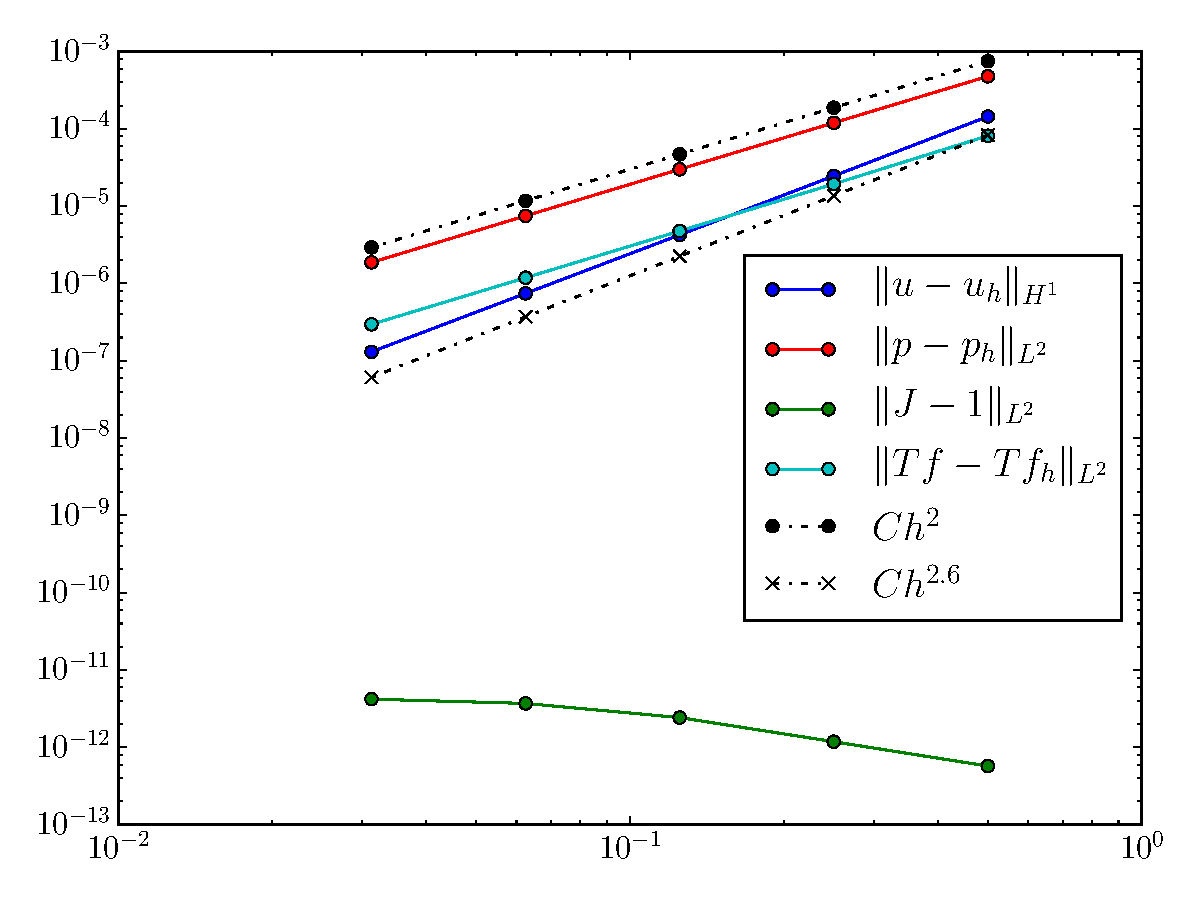
\includegraphics[width=\textwidth]{figures/mms2d_active_stress}
     \caption{\label{fig:mms2d_active_stress}Active stress}
\end{subfigure}
% \qquad
\begin{subfigure}[t]{0.3\textwidth}
    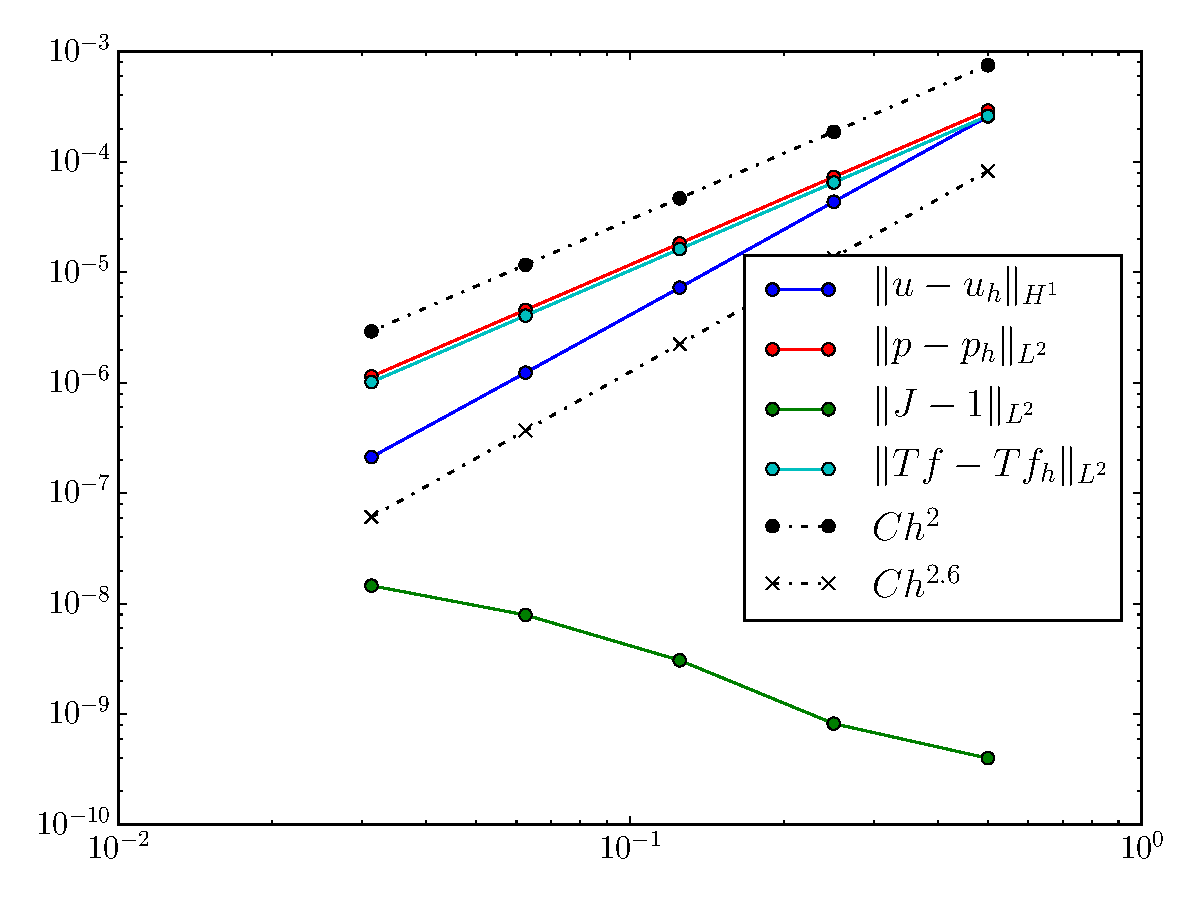
\includegraphics[width=\textwidth]{figures/mms2d_active_strain_rossi}
    \caption{\label{fig:mms2d_active_stain_rossi}Active strain \eqref{eq:active_strain_Fa_rossi} }    
\end{subfigure}
% \qquad
\begin{subfigure}[t]{0.3\textwidth}
    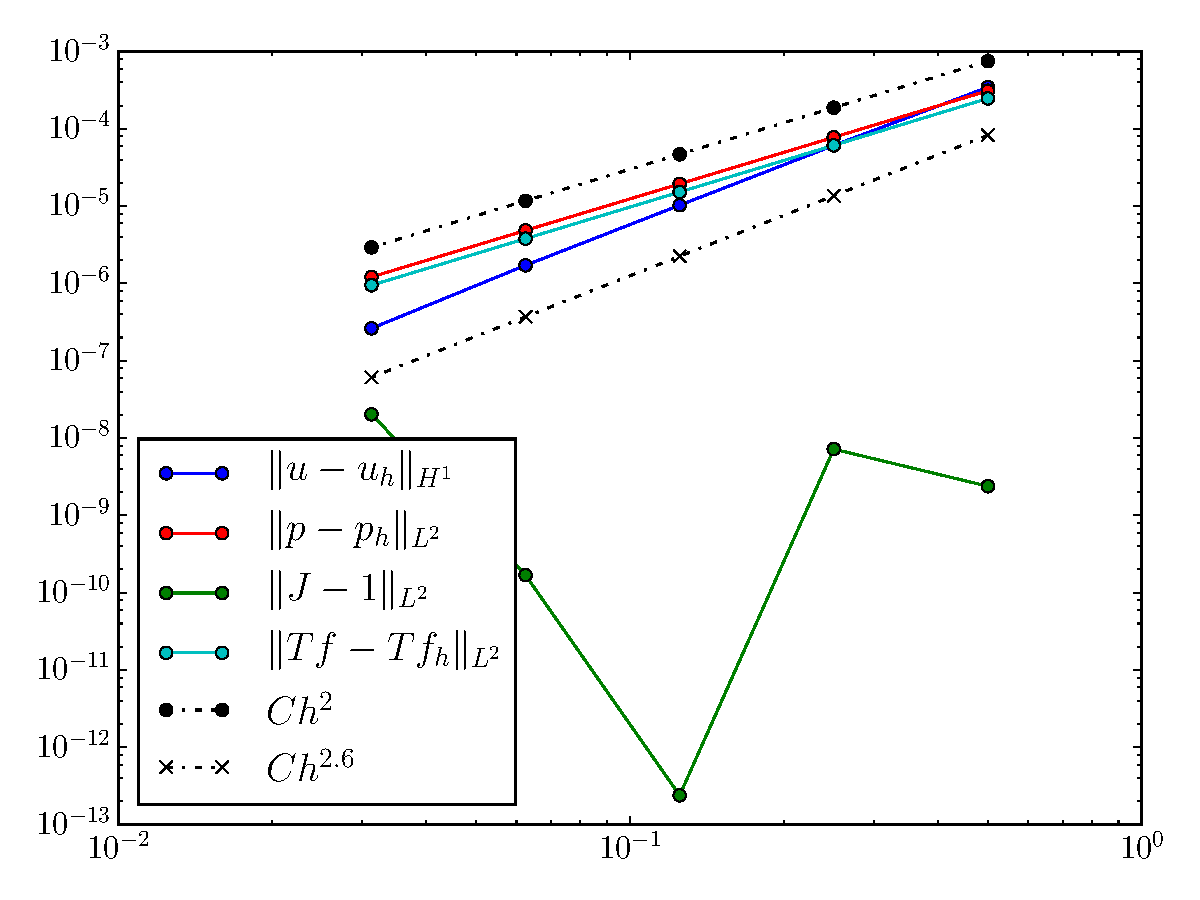
\includegraphics[width=\textwidth]{figures/mms2d_active_strain}
    \caption{\label{fig:mms2d_active_stain_gjerald}Active strain \eqref{eq:active_strain_Fa_gjerald} }    
\end{subfigure}
\label{fig:mms2d_convergence_inc}
\caption{Convergence of displacement $\uvec$, hydrostatic pressure $p$, determinant of the deformation gradient $J$ and fiber stress $Tf$.}  
\end{figure}

It should be noted that in the case illustrated in Figure \ref{fig:mms2d_convergence_inc} we have not removed volumetric strains
from the strain energy. Removing these volumetric straines, i.e using the formulation in \eqref{eq:quasi-incompressible}
we do not get the desired convergence as can be seen from Figure \ref{fig:mms2d_convergence_qinc}. As we can see, we do not get convergence of the Lagrange multiplier $p$. However, when useing the formulation \eqref{eq:active_strain_Fa_gjerald}, we see from Figure \ref{fig:mms2d_active_stain_gjerald_qinc} that we get infact convergence of th displacement and the fiber stress. Strange...

\begin{figure}[htbp]
\centering
\begin{subfigure}[t]{0.3\textwidth}
     \centering
     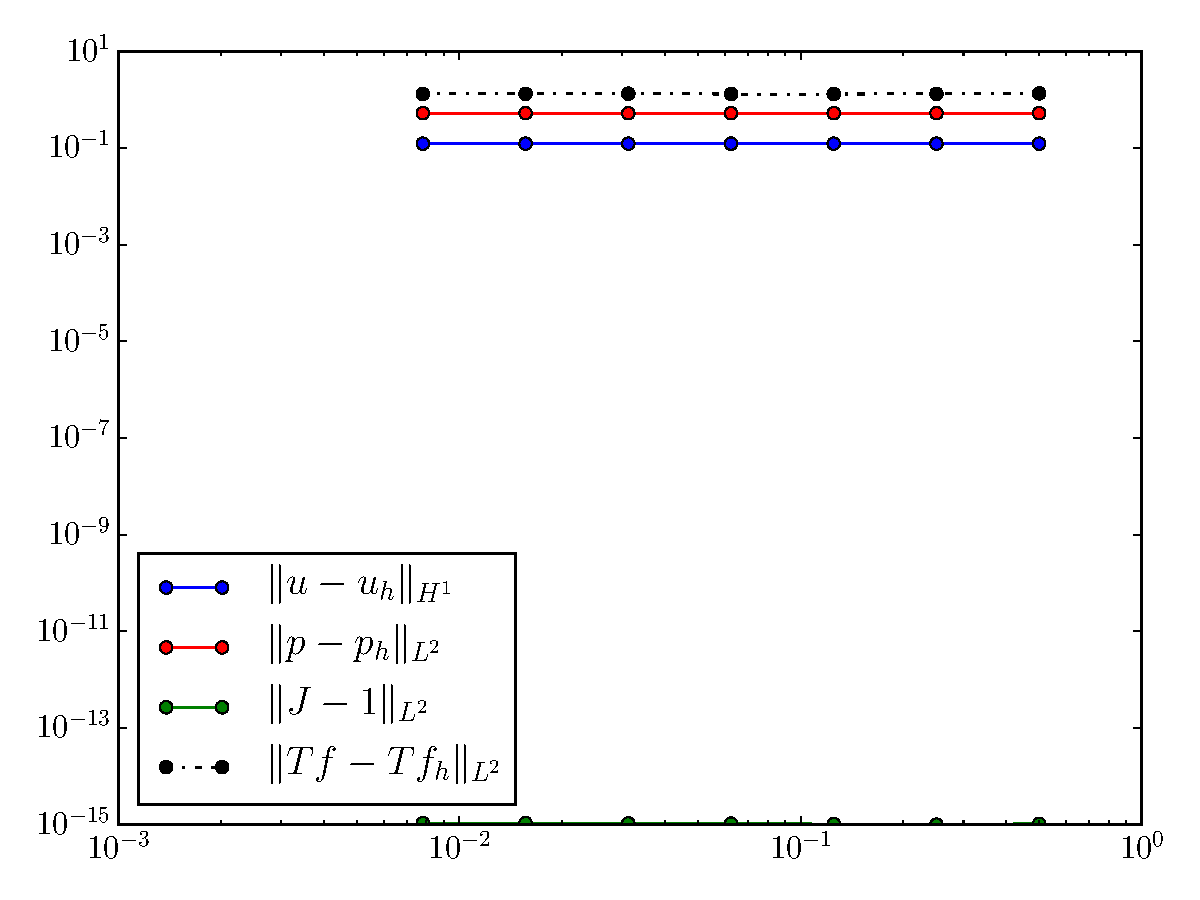
\includegraphics[width=\textwidth]{figures/mms2d_active_stress_qinc}
     \caption{\label{fig:mms2d_active_stress_qinc}Active stress}
\end{subfigure}
% \qquad
\begin{subfigure}[t]{0.3\textwidth}
    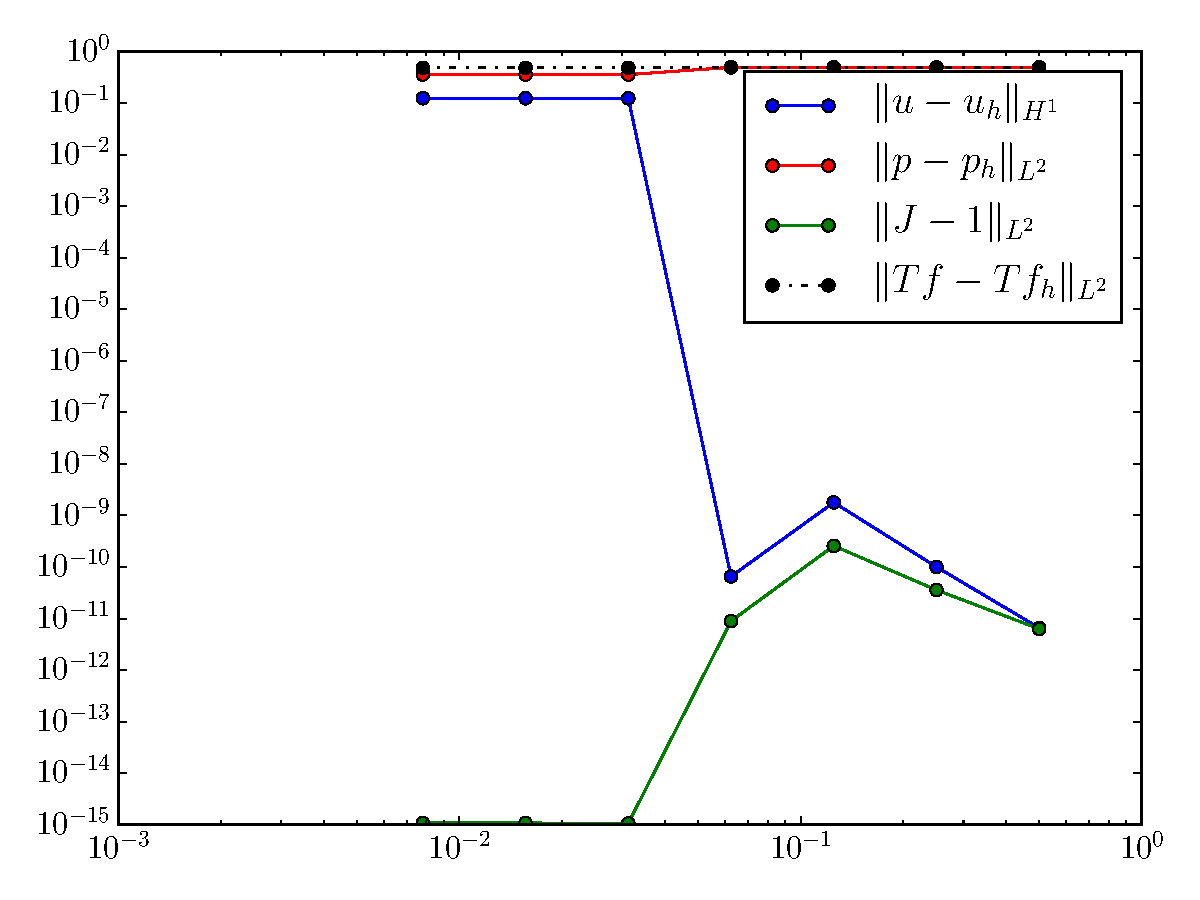
\includegraphics[width=\textwidth]{figures/mms2d_active_strain_rossi_qinc}
    \caption{\label{fig:mms2d_active_stain_rossi_qinc}Active strain \eqref{eq:active_strain_Fa_rossi} }    
\end{subfigure}
% \qquad
\begin{subfigure}[t]{0.3\textwidth}
    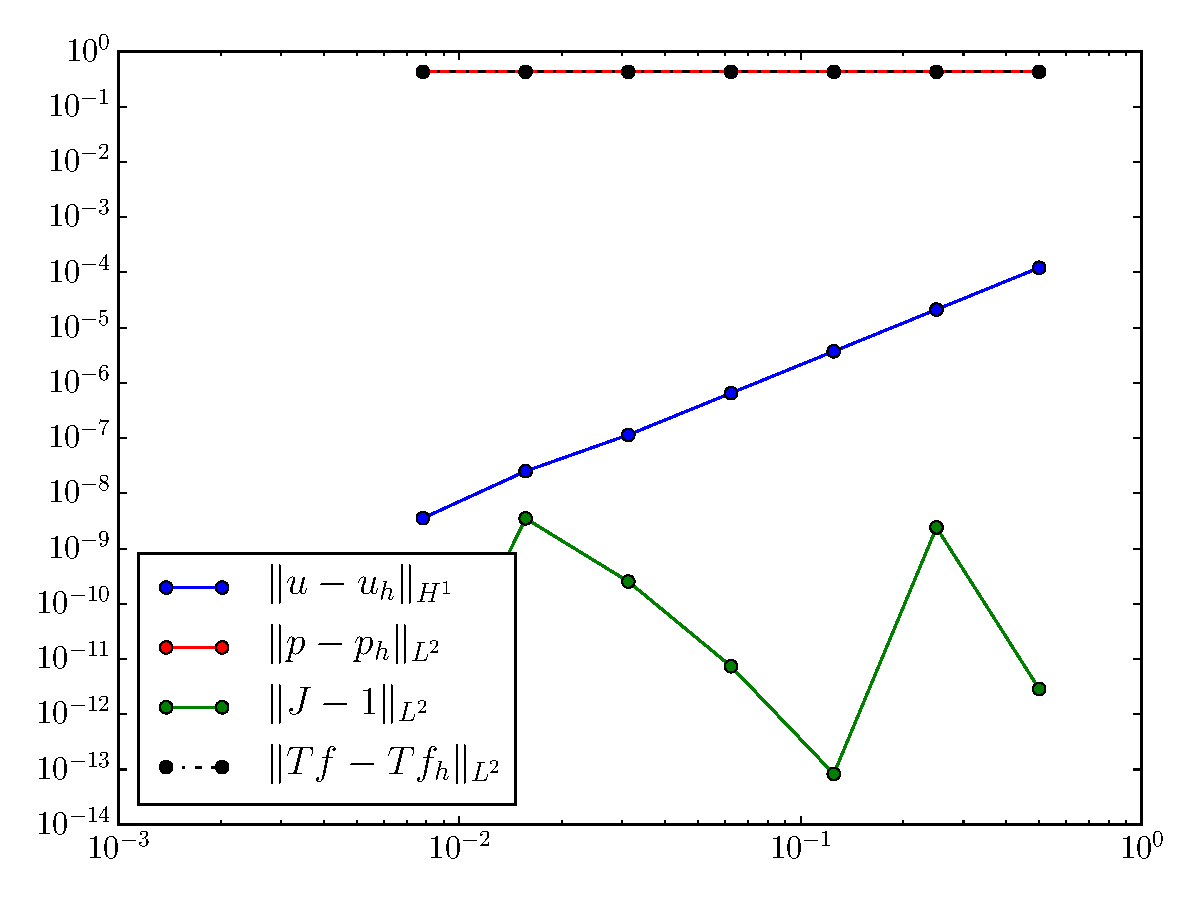
\includegraphics[width=\textwidth]{figures/mms2d_active_strain_qinc}
    \caption{\label{fig:mms2d_active_stain_gjerald_qinc}Active strain \eqref{eq:active_strain_Fa_gjerald} }    
\end{subfigure}
\caption{\label{fig:mms2d_convergence_qinc}Convergence of displacement $\uvec$, hydrostatic pressure $p$, determinant of the deformation gradient $J$ and fiber stress $Tf$ when volumetric strain are removed.}  
\end{figure}




\bibliographystyle{plain}
\bibliography{bibliography}
\end{document}

%%% Local Variables:
%%% mode: latex
%%% TeX-master: t
%%% End:
